\documentclass[10pt]{article}

%==============================
% Document Metadata
%============================== 
\usepackage[pdftex,
    pdfauthor={Rukmal Weerawarana},
    pdftitle={Homework 1 Solutions - FE 621},
    pdfsubject={FE 621 - Computational Methods in Finance}
]{hyperref}


%==============================
% Package Imports
%==============================    
\usepackage[ruled]{algorithm2e} % typeset algorithms
\usepackage[authordate, maxcitenames=1]{biblatex-chicago} % chicago bibliography style
\usepackage{amsmath} % math environment stuff
\usepackage{amssymb} % additional math symbols
\usepackage[toc, page]{appendix} % Appendix referencing
\usepackage{booktabs} % Table lines
\usepackage{comment} % enables the use of multi-line comments (\ifx \fi)
\usepackage[skip=5pt, labelfont=bf]{caption} % caption formatting
\usepackage{csvsimple} % CSV import to Table
\usepackage{fancyhdr} % Header
\usepackage{fancyvrb} % Verbatim text
\usepackage{float} % Controlling figure border
\usepackage[headings]{fullpage} % Set all margins to 1.5 cm
\usepackage{graphicx} % Figures
\usepackage{listings} % code embedding
\usepackage{longtable} % Multipage tables
\usepackage{multirow} % Multirow cells in tables
\usepackage{pmboxdraw} % Box characters for file tree
\usepackage[dvipsnames]{xcolor} % colors for code


%==============================
% Configuration
%==============================

% Figure outline configuration
% \floatstyle{boxed}
% \restylefloat{figure}

% Bibliography configuration

\addbibresource{../bibliography.bib}

% Remapping bibliography underscores (_) and tildes (~) because Mendeley has weird exporting
% Solution from: https://tex.stackexchange.com/questions/309980/parsing-underscores-in-urls-from-mendeley

\DeclareSourcemap{ % Used when .bib/Bibliography is compiled, not when document is
    \maps{
        \map{ % Replaces '{\_}', '{_}' or '\_' with just '_'
            \step[fieldsource=url,
                  match=\regexp{\{\\\_\}|\{\_\}|\\\_},
                  replace=\regexp{\_}]
        }
        \map{ % Replaces '{'$\sim$'}', '$\sim$' or '{~}' with just '~'
            \step[fieldsource=url,
                  match=\regexp{\{\$\\sim\$\}|\{\~\}|\$\\sim\$},
                  replace=\regexp{\~}]
        }
    }
}

% Code display configuration

\newcommand*\lstinputpath[1]{\lstset{inputpath=#1}} % Setting path
\lstset{
	language=Python,
	basicstyle=\footnotesize\ttfamily,
	commentstyle=\ttfamily\color{purple!40!black},
	identifierstyle=\color{blue},
	keywordstyle=\color{ForestGreen},
	numbers=left,
	numberstyle=\ttfamily\color{gray}\footnotesize,
	stepnumber=1,
	numbersep=5pt,
	backgroundcolor=\color{white},
	showspaces=false,
	showstringspaces=false,
	showtabs=false,
	frame=single,
	tabsize=2,
	captionpos=b,
	breaklines=true,
	breakatwhitespace=false,
	title=\lstname
}
\lstset{
	language=R,
	basicstyle=\footnotesize\ttfamily,
	commentstyle=\ttfamily\color{purple!40!black},
	identifierstyle=\color{blue},
	keywordstyle=\color{ForestGreen},
	numbers=left,
	numberstyle=\ttfamily\color{gray}\footnotesize,
	stepnumber=1,
	numbersep=5pt,
	backgroundcolor=\color{white},
	showspaces=false,
	showstringspaces=false,
	showtabs=false,
	frame=single,
	tabsize=2,
	captionpos=b,
	breaklines=true,
	breakatwhitespace=false,
	title=\lstname
}

% Header and Footer configuration

\pagestyle{fancy} % set page style
\fancyhead{} % override header
\fancyfoot{} % override footer
\renewcommand{\headrulewidth}{.4pt} % set header rule width 
\renewcommand{\footrulewidth}{.4pt} % set footer rule width 
\lhead{Homework Assignment 2} % set left header
\rhead{Rukmal Weerawarana} % set right header
\lfoot{\textit{FE 621}: Computational Methods in Finance} % set left footer
\rfoot{Page \thepage} % set right footer


%==============================
% Document Content
%==============================

\begin{document}

\thispagestyle{plain}

\pagenumbering{roman}  % Changing numbering to Roman numerals for first pages

%==============================
% Document Title
%==============================

\noindent
\large\textbf{Homework Assignment 2} \hfill \textbf{Rukmal Weerawarana} \\
\normalsize \textit{FE 621}: Computational Methods in Finance \hfill \textit{rweerawa@stevens.edu} $\mid$ 104-307-27 \\
\textit{Instructor}: Ionut Florescu \hfill Department of Financial Engineering \\
3/25/2019 \hfill Stevens Institute of Technology

\noindent\rule{\linewidth}{.1em}


%==============================
% Overview
%==============================

\section*{Overview}

In this Homework Assignment, we explore various numerical optimization methods through the lens of the Black-Scholes-Merton Option pricing model\footnote{\cite{Shreve2004}}. Using this, we calculate and explore the implied volatility of options for various assets traded on the market. Furthermore, we also explore numeric methods of differential calculation to compute the Greeks of these candidate options. Finally, we explore numeric integration and the behavior of various quadrature methods.

Unless otherwise stated, the following shorthand notation is used to distinguish between dates:

\begin{itemize}
    \item \textbf{DATA1} - Wednesday, February 6 2019 (\textit{2/6/19});
    \item \textbf{DATA2} - Thursday, February 7 2019 (\textit{2/7/19}).
\end{itemize}

The content of this Homework Assignment is divided into three sections; the first discusses data gathering, formatting, and a discussion of the assets being examined. The second contains data analysis, and an exploration of implied volatility through the Black-Scholes-Merton pricing framework and related computations. Finally, the third section discusses numerical integration and the convergence of various quadrature rules.

\begin{center}
    \textit{See Appendix~\ref{appendix:source} for specific question implementations, and the project GitHub repository\footnote{\cite{Weerawarana2019}} for full source code of the {\normalfont \texttt{fe621}} Python package.}
\end{center}


%==============================
% Table of Contents
%==============================

\newpage

\tableofcontents

%==============================
% Section 1
%==============================

\newpage

\pagenumbering{arabic}  % Changing numbering to arabic numerals for main content

\section{Tree Implementation}

    \subsection{General Tree Construction}

    To simplify the construction of all tree-like structures, I implemented a fully generalized tree structure. This structure handles tree construction and traversal, completely encapuslating all required functionality.

    The class intelligently exposes price and value tree variables during traversal, and abstract methods are designed to be overridden to implement a specific tree pricing algorithm. This general tree class is reproduced below. Furthermore, the class also utilizes DOK (i.e. \textit{Dictionary-of-Keys}) matrices whenever possible. This provides quick \textit{O(1)} access to elements, and minimizes overall space complexity, as zero-valued fields are not store explicitly.

        \lstinputlisting{../fe621/tree_pricing/general_tree.py}
    

    \newpage
    \subsection{Binomial Tree}

    Following this implementation strategy, the additive Trigeorgis\cite{Trigeorgis1991} tree was implemented. Required methods of the abstract \texttt{GeneralTree} class were overridden to implement the Trigeorgis tree for both Call and Put options, of both American and European options in a single class.

    Furthermore, optimizations were made to the Trigeorgis tree class, such that a European option can be computed from the same price tree as constructed for an American option, and vice versa. This functionality enables efficient cross-style option value computations with minimal space complexity.

    The Trigeorgis tree implementation is reproduced below.

        \lstinputlisting{../fe621/tree_pricing/binomial/trigeorgis.py}

    \newpage
    \subsection{Trinomial Tree}

    
    Similar to the Trigeorgis tree above, a generalized additive Trinomial tree was implemented utilizing the same abstract \texttt{GeneralTree} class. The implementation of a Trinomial tree utilizing the same abstract class illustrates its versatility, with constructed DOK price and value trees intelligently adapting to the different degree of the tree.
    
    This was accomplished entirely by overriding prescribed abstract methods of the \texttt{GeneralTree} class, without any direct modification of the generalized tree class. The Trinomial Additive Tree implementation is reproduced below.

    \lstinputlisting{../fe621/tree_pricing/trinomial/trinomial_price.py}
    
\newpage
\section{Binomial Tree Operations}

    \subsection{Computed Option Prices}

    Option prices were computed, utilizing data from Homework Assignment 1's SPY \textbf{DATA2} dataset. To begin, both American and European style options were computed for options of various strike prices, with expiration dates varying from 1 to 3 months of the data gathering date.

    This data is reproduced in Appendix~\ref{appendix:q1:binomial_prices}, and the source code for this computation is reproduced in Appendix~\ref{appendix:q1:binomial_prices}.

    As seen in the tables, the computed values for the European style option with the Binomial tree agree with the analytically computed Black Scholes price. This behavior is to be expected, as the Binomial Tree price converges to the Black Scholes price as the step size, $N \rightarrow \infty$.

    Furthermore, it can also be noted that the prices of the American style options are consistently higher. Note that some significant figures may be truncated in the presentation of the table in this document.
    
    This behavior is also expected. Under the efficient market hypothesis, and the risk-neutral assumption of option pricing, risk is compensated equally. Thus, the higher cost of the American style options can be attributed to the fact that the holder must pay for the \textit{optionality} provided by the early-exercise feature of American style options, compared to their European style counterparts.


    \subsection{Absolute Error Analysis}
    
    To better understand the behavior of the Binomial Tree pricing under varying step sizes, the following error function was plotted for various values of the step size, $N$. The source code for this computation is reproduced in Appendix~\ref{appendix:source:q1:abs_error}.

    \begin{gather*}
        N \in \{10, 20, 30, 40, 50, 100, 150, 200, 250, 300, 350, 400\} \\
        \\
        \epsilon_N = \left| P^{BSM}(\cdot) - P^{BTree}_N(\cdot) \right|
    \end{gather*}

    \begin{table}[!h]
        \centering
        \csvautotabular{bin/binomial_tree_abs_error.csv}
        \caption{Absoute error of Binomial Tree Put Option price computation, with respect to a range of varying step sizes, $N$.}
        \label{table:binomial_abs_error}
    \end{table}

    Where $P^{BTree}_N$ is the price of a put option computed with a binomial tree of $N$ steps. The table of absolute errors is reproduced in Table~\ref{table:binomial_abs_error}. Additionally, a graphical representation of this data is also presented in Figure~\ref{fig:binomial_abs_error}.

    \begin{figure}[!ht]
        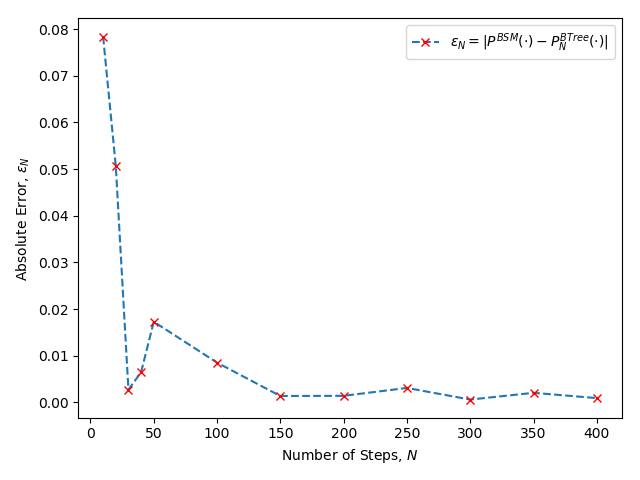
\includegraphics[]{bin/binomial_abs_error_plot.png}
        \caption{Absolute error analysis of the Binomial Tree price computation convergence, with respect to varying step sizes.}
        \label{fig:binomial_abs_error}
    \end{figure}

    As evidenced by the graphic, there is a clear pattern of convergence to a the analytically computed value as the number of steps, $N$ increases. This is to be expected, as at the limit as $N \rightarrow \infty$, the Binomial Tree process will perfectly approximate a continuous geometric brownian motion.

    \newpage
    \subsection{Implied Volatility Computation}
    
    Following the algorithm outlined in Homework 1, I computed the implied volatility for the selection of option contracts used in this Homework Assignment, using the Binomial Option Tree, driven by a Bisection Search Algorithm. Source code for this computation is reproduced in Appendix~\ref{appendix:source:q1:imp_vol}.

    Compared to the implied volatilities computed in Homework Assignment 1, the volatilities computed here are marginally higher. This too can be attributed to the fact that the holder is compensated fairly for the added optionality provided under the American Option heuristic, used in this computation.

%==============================
% References
%==============================

\newpage

\printbibliography

%==============================
% APPENDIX
%==============================

\newpage

\appendix

% Resetting input path
\lstinputpath{}

\section{Binomial Tree Option Prices} \label{appendix:q1:binomial_prices}

    \csvreader[
        longtable=l|ccccc,
        table head=
            \toprule\bfseries Option Name &\bfseries Strike &\bfseries Implied Volatility &\bfseries Binomial (A) &\bfseries Binomial (E) &\bfseries BS (E) \\ \midrule \endhead \bottomrule \endfoot,
        late after line=\\
    ]{bin/binomial_data2_prices.csv}{1=\one, 2=\two, 3=\three, 4=\four, 5=\five, 6=\six, 7=\seven}{\one & \seven & \five & \two & \three & \four}

\newpage
\section{Binomial Tree Implied Volatility} \label{appendix:q1:imp_vol}

    \csvreader[
        longtable=l|ccc,
        table head=
            \toprule\bfseries Option Name &\bfseries Strike &\bfseries Type &\bfseries Binomial Implied Volatility \\ \midrule \endhead \bottomrule \endfoot,
        late after line=\\
    ]{bin/binomial_implied_vol.csv}{1=\one, 2=\two, 3=\three, 4=\four}{\one & \three & \three & \two}

\newpage
\section{Trinomial Tree Option Prices} \label{appendix:q2:trinomial_prices}

    \csvreader[
        longtable=l|ccccc,
        table head=
            \toprule\bfseries Option Name &\bfseries Strike &\bfseries Implied Volatility &\bfseries Trinomial (A) &\bfseries Trinomial (E) &\bfseries BS (E) \\ \midrule \endhead \bottomrule \endfoot,
        late after line=\\
    ]{bin/trinomial_data2_prices.csv}{1=\one, 2=\two, 3=\three, 4=\four, 5=\five, 6=\six, 7=\seven}{\one & \five & \three & \six & \seven & \two}

\newpage
\section{Trinomial Tree Implied Volatility} \label{appendix:q2:imp_vol}

    \csvreader[
        longtable=l|ccc,
        table head=
            \toprule\bfseries Option Name &\bfseries Strike &\bfseries Type &\bfseries Binomial Implied Volatility \\ \midrule \endhead \bottomrule \endfoot,
        late after line=\\
    ]{bin/trinomial_implied_vol.csv}{1=\one, 2=\two, 3=\three, 4=\four}{\one & \two & \four & \three}

\newpage
\section{Solution Source Code} \label{appendix:source}

    \subsection{Question 1 Implementation} \label{appendix:source:q1}

        \subsubsection{Binomial Tree Price Computation} \label{appendix:source:q1:prices}

            \lstinputlisting{question_solutions/question_1_prices.py}
        
        \subsubsection{Binomial Tree Absolute Error Analysis} \label{appendix:source:q1:abs_error}

            \lstinputlisting{question_solutions/question_1_abs_error.py}
        
        \subsubsection{Binomial Tree Implied Volatility Optimization} \label{appendix:source:q1:imp_vol}

            \lstinputlisting{question_solutions/question_1_imp_vol.py}

    \newpage
    \subsection{Question 2 Implementation} \label{appendix:source:q2}

        \subsubsection{Trinomial Tree Price Computation} \label{appendix:source:q2:prices}

            \lstinputlisting{question_solutions/question_2_prices.py}
        
        \subsubsection{Trinomial Tree Absolute Error Analysis} \label{appendix:source:q2:abs_error}

            \lstinputlisting{question_solutions/question_2_abs_error.py}
        
        \subsubsection{Trinomial Tree Implied Volatility Optimization} \label{appendix:source:q2:imp_vol}

            \lstinputlisting{question_solutions/question_2_imp_vol.py}

    
%==============================
% Document End
%==============================

\end{document}
